\chapter{Diseño e implementación}
\label{Chapter3}

En el presente capítulo se describe el diseño e implementación del sistema desarrollado. Se presentan la arquitectura general de hardware y software, los criterios utilizados para la selección de componentes y las principales decisiones de diseño adoptadas durante el desarrollo. Asimismo, se detallan la estructura del firmware, las comunicaciones implementadas y la integración entre los distintos módulos del sistema.

%----------------------------------------------------------------------------------------
\section{Arquitectura del sistema}
La figura \ref{fig:arquitectura_general} presenta la arquitectura general del sistema desarrollado. La solución se compone de una estación central conectada mediante Ethernet TCP/IP a la interfaz de usuario y múltiples estaciones remotas enlazadas de forma inalámbrica mediante IEEE 802.15.4. Cada estación remota interactúa con variables de proceso asociadas a sensores, actuadores e interfaces industriales.

\begin{figure}[ht]
	\centering
	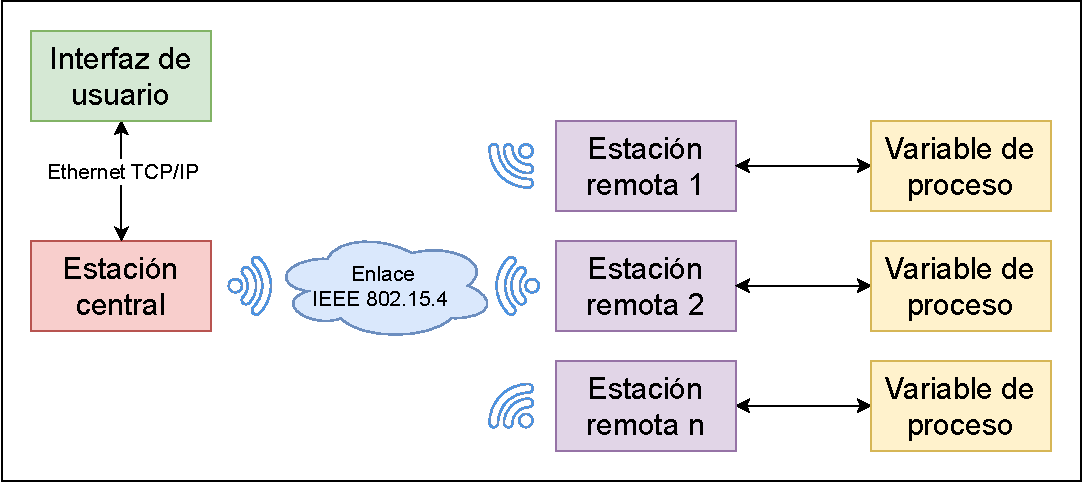
\includegraphics[width=1.0\textwidth]{./Figures/arquitectura_general.pdf}
	\caption{Arquitectura general del sistema implementado.}
	\label{fig:arquitectura_general}
\end{figure}

\subsection{Diagrama de bloques del hardware}

La figura \ref{fig:arquitectura_hardware} presenta el diagrama de bloques del hardware desarrollado. La arquitectura se basa en un microcontrolador encargado de gestionar las interfaces de comunicación, las entradas y salidas industriales y los módulos auxiliares del sistema. Asimismo, se distinguen los bloques comunes a las estaciones centrales y remotas y aquellos específicos de cada tipo de nodo.

Con el objetivo de uniformar el desarrollo y reducir costos durante una etapa inicial del trabajo, se implementó un único diseño de placa de circuito impreso PCB (\textit{Printed Circuit Board}, Placa de Circuito Impreso) tanto para las estaciones centrales como para las estaciones remotas. Esta estrategia permitió reutilizar el mismo diseño base de hardware y poblar únicamente los componentes requeridos según las funcionalidades de cada estación. Además de simplificar el proceso de desarrollo, esta decisión redujo los costos de fabricación y facilitó las tareas de validación y mantenimiento del sistema.

La estación central incorpora un transceptor Ethernet para la comunicación con una interfaz de usuario ubicada en un nivel jerárquico superior. Asimismo, dispone de un reloj de tiempo real RTC (\textit{Real-Time Clock}, Reloj de Tiempo Real), utilizado para el registro y mantenimiento de fecha y hora ante interrupciones en la alimentación principal.

Por otro lado, las estaciones remotas incorporan una interfaz RS485 para la comunicación con instrumentos industriales y módulos de entradas y salidas digitales destinados a la adquisición y accionamiento de variables de proceso.

Tanto las estaciones centrales como las remotas comparten los módulos de alimentación y regulación de tensión, el microcontrolador principal y el transceptor inalámbrico IEEE 802.15.4 utilizado para la comunicación entre nodos.

\begin{figure}[ht]
	\centering
	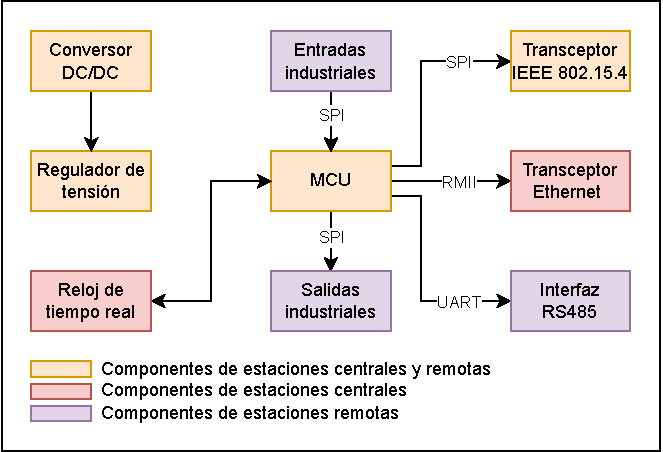
\includegraphics[width=1.0\textwidth]{./Figures/arquitectura_hardware.pdf}
	\caption{Diagrama de bloques general del hardware.}
	\label{fig:arquitectura_hardware}
\end{figure}

\subsection{Diagrama de bloques del firmware}
La figura \ref{fig:arquitectura_firmware} presenta la arquitectura general del firmware implementado en el sistema. Este fue organizado en capas con el objetivo de desacoplar la lógica de aplicación de las dependencias específicas del hardware y facilitar la reutilización de código entre estaciones centrales y remotas.

La capa superior contiene la lógica de control y supervisión del sistema. Por debajo se ubica una API (\textit{Application Programming Interface}, Interfaz de Programación de Aplicaciones) encargada de abstraer el acceso a sensores, actuadores e interfaces del sistema. Las capas intermedias incorporan los servicios de middleware, incluyendo el sistema operativo en tiempo real FreeRTOS y la pila de comunicaciones lwIP. Finalmente, las capas inferiores contienen los controladores de periféricos, la capa de abstracción de hardware HAL (\textit{Hardware Abstraction Layer}, Capa de Abstracción de Hardware) y los módulos físicos del sistema.

\begin{figure}[ht]
	\centering
	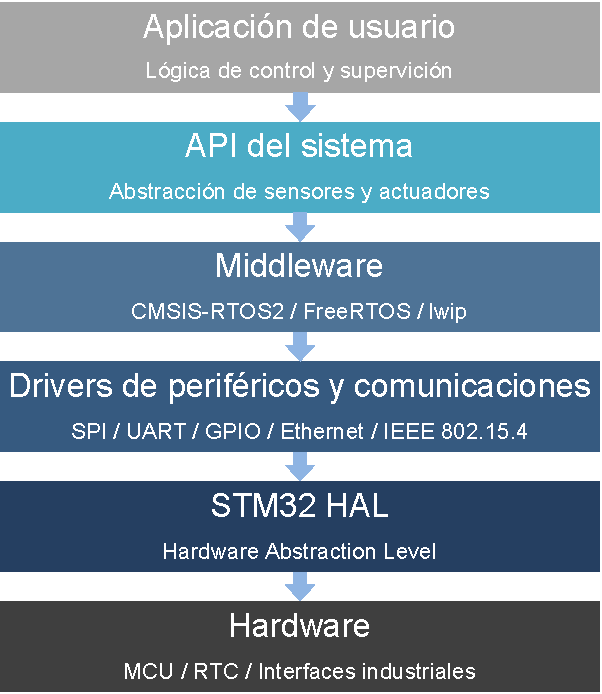
\includegraphics[width=0.7\textwidth]{./Figures/arquitectura_firmware.pdf}
	\caption{Diagrama de bloques general del firmware.}
	\label{fig:arquitectura_firmware}
\end{figure}
